\documentclass[14pt,aspectratio=1610]{beamer}
%\documentclass[12pt,aspectratio=1610,handout]{beamer}
\usepackage{csu-theme}
\usepackage{arrays}
\usepackage{algpseudocode}
\usepackage{booktabs}

\title{{\Huge{} Graphs}\\{\LARGE{} via Adjacency Matrices}}
\subtitle{CSCI 315: Data Structure Analysis\\Chapter 20}
\author{Sean T. Hayes, Ph.D.}
\institute{Charleston Southern University}

%% Comment out date to use default (today)
% \date{April 8, 2025}
\subject{Software Programming}
%\keywords{}

\setlength{\parskip}{0.5em}

\graphicspath{{../imgs/}{../imgs/graphs}}

\usepackage{tikz}
\usetikzlibrary{arrows,automata}

\tikzset{
  every state/.style={minimum size=12pt, inner sep=4pt, fill=CSUcyan, text=black, very thick},
  marked/.style={text=white, fill=CSUslate},
  visit/.style={text=black, fill=CSUgold},
  %->,
  >=stealth',
  auto,
  node distance=1.5cm,
  font=\ttfamily,
  % main node/.style={circle,draw,font=\ttfamily\bfseries,minimum size=0pt, inner sep=2pt},
  every text node part/.style={align=center},
  %
  % Used for Beamer overlays
  invisible/.style={opacity=0,text opacity=0},
  visible on/.style={alt=#1{}{invisible}},
  alt/.code args={<#1>#2#3}{%
    \alt<#1>{\pgfkeysalso{#2}}{\pgfkeysalso{#3}} % \pgfkeysalso doesn't change the path
  },
}

% Used to stylize 0 in the adjacency matrix
\newcommand{\mFal}[1][0]{\texttt{\textcolor{CSUgold}{#1}}}
\newcommand{\mTru}[1][1]{\texttt{\textbf{#1}}}

\newcommand{\vertMark}[1][CSUgold]{full=#1}

\newcommand{\textInf}{$\infty$}

\newcommand{\arraySubscript}[1]{\texttt{\textcolor{white!75!CSUblue}{[}{#1}\textcolor{white!75!CSUblue}{]}}}


\begin{document}

\begin{frame}
  \titlepage
\end{frame}

\section*{Intro}
\begin{frame}{K{\"o}nigsberg Bridge Problem}
The river Pregel flows around the island of Kneiphof\\
and then divides into two branches.

\vspace{0.5em}
\centerline{%
  
\includegraphics[width=0.6\textwidth]{Konigsberg-Euler}
}

Starting at one land area, can you cross all 7 bridges exactly once and return to the start?
\end{frame}

\begin{frame}{K{\"o}nigsberg Bridge Problem}
In 1736, Euler invented graph theory by representing this problem as a graph to solve the problem.
\begin{columns}
\column{0.6\textwidth}
%\begin{figure}
  \centerline{%
    
\includegraphics[width=0.9\textwidth]{Konigsberg-Euler}
  }
%\end{figure}
\column{0.4\textwidth}
\pause{}
\centerline{%
  \begin{tikzpicture}[very thick]
    \node[state] (A)                    {A};
    \node[state]         (C) [above of=A] {C};
    \node[state]         (B) [below of=A] {B};
    \node[state]         (D) [right of=A, node distance=3cm] {D};

    \path (A) edge [bend left]  node {b} (B)
              edge [bend left]  node {c} (C)
              edge              node {e} (D)
          (B) edge [bend left]  node {a} (A)
              edge              node [below]{f} (D)
          (C) edge [bend left]  node {d} (A)
              edge              node {g} (D);
  \end{tikzpicture}%
}
\end{columns}
\pause{}
Euler determined that only 0 or 2 vertices (lands) can have an odd number of edges (bridges). All 4 lands have an odd number of bridges, so there is no solution.
\end{frame}

\begin{frame}{Graph Theory}
Over the past 250 years, graph theory has been applied \\
to a variety of problems, including:
\begin{itemize}
  \item  modeling and analysis of electrical circuits,
  \item  chemical compounds,
  \item  highway maps,
  \item  finding the shortest route,
  \item  project planning,
  \item  linguistics,
  \item  genetics,
  \item  social science,
  \item  etc.
\end{itemize}
\end{frame}

\section{Notation}

\begin{frame}{Set Theory Notation}
\begin{itemize}
  \item
    \emph{Member} ($x \in A$): $x$ is an element of the set $X$.
  \item
    \emph{Subset} ($A \subseteq B$): every element of $A$ is an element of $B$.
  \item
    \emph{Intersection} ($A \cap B$): contains all the elements in $A$ and $B$.\\
    $A \cap B = \{x \mid x \in A$ and $x \in B\}$
  \item
    \emph{Union} ($A \cup B$): set of all the elements that are in $A$ or in $B$.\\
    $A \cup B = \{x \mid x \in A$ or $x \in B\}$
  \item
    \emph{Ordered Pairs} ($A \times B$): set of all the ordered pairs of elements of $A$ and $B$.\\
    $A \times B = \{(a, b) \mid a \in A, b \in B\}$

\end{itemize}
\end{frame}

\begin{frame}{Graph Definitions and Notations}
\emph{Graph} $G \mid G = (V, E)$
\begin{itemize}
  \item
    $V$ is a finite nonempty set of \emph{vertices} of $G$.
  \item
    $E \subseteq V \times V$.\\
    Elements in $E$ are the pairs of elements of $V$.\\
    $E$ is the set of \emph{edges}.
\end{itemize}
\end{frame}

\begin{frame}{Directed Graphs}
\emph{Directed graph} or \emph{digraph}: elements of \(E(G)\) are ordered pairs.
\begin{itemize}
  \item
    Pairs ($u$, $v$) and ($v$, $u$) represent different edges.
\end{itemize}
\begin{columns}
\column{0.5\textwidth}
\begin{figure}
\centering
\begin{tikzpicture}[very thick, ->, shorten >=0.5pt]
  \node[state] (A)                      {A};
  \node[state]         (B) [right of=A] {B};

  \node[state]         (D) [below of=A] {C};
  \node[state]         (E) [right of=D] {D};
  \node[state]         (C) [right of=E] {E};

  \path (A) edge [bend right] (B)
            edge (D)
        (B) edge (C)
            edge [bend right] (A)
            edge (E)
        (D) edge [bend right] (C)
            edge (E);
\end{tikzpicture}
\end{figure}
\column{0.5\textwidth}
  \begin{figure}
  \centering
  \begin{tikzpicture}[very thick, ->, shorten >=0.5pt]
    \node[state] (0)              {0};
    \node[state] (1) [right of=0] {1};
    \node[state] (2) [right of=1] {2};
    \node[state] (3) [right of=2] {3};
    \node[state] (4) [below of=0] {4};
    \node[state] (5) [right of=4] {5};
    \node[state] (6) [right of=5] {6};
    \node[state] (7) [below of=4] {7};
    \node[state] (8) [right of=7, node distance=3cm] {8};

    \path (0) edge (1)
              edge (4)
          (1) edge (2)
              edge (6)
          (2) edge [bend right] (0)
              edge (3)
          (4) edge (5)
              edge (7)
          (5) edge (8)
          (6) edge (5)
          (7) edge [bend left] (0)
          (8) edge (7)
              edge (6);
  \end{tikzpicture}
\end{figure}
\end{columns}
\end{frame}


\begin{frame}{Undirected Graphs}
\begin{itemize}
  \item
    \emph{Undirected graph}: elements are not ordered pairs.
    \begin{itemize}
      \item
        Pairs ($u$, $v$) and ($v$, $u$) represent the same edge.
    \end{itemize}
\end{itemize}

\begin{columns}
\column{0.5\textwidth}
\begin{figure}
\centering
\begin{tikzpicture}[very thick]
    \node[state] (0)              {0};
    \node[state] (1) [right of=0] {1};
    \node[state] (2) [right of=1] {2};
    \node[state] (3) [below of=0] {3};
    \node[state] (4) [right of=3] {4};
    \node[state] (5) [right of=4] {5};
    \node[state] (6) [below of=5] {6};

    \path (0) edge (1)
              edge [bend left] (2)
              edge (3)
              edge (4)
          (1) edge (4)
          (3) edge (4)
              edge (6)
          (4) edge (5)
          (5) edge (6)
          (6) edge [bend right] (2);
\end{tikzpicture}
\end{figure}
\column{0.5\textwidth}

\begin{figure}
\centering
\begin{tikzpicture}[very thick]
    \node[state] (0)              {0};
    \node[state] (1) [below left of=0, xshift=-0.75cm] {1};
    \node[state] (2) [below right of=0, xshift=0.75cm] {2};
    \node[state] (3) [below right of=1] {3};
    \node[state] (4) [below left of=2] {4};
    \node[state] (5) [below right of=2] {5};
    \node[state] (6) [below left of=5] {6};

    \path (0) edge (1)
              edge (2)
          (1) edge (3)
          (2) edge (4)
              edge (5)
          (5) edge (6);
\end{tikzpicture}
\end{figure}
\end{columns}
\end{frame}

\begin{frame}{Undirected Graphs}
\begin{figure}
\centering
\begin{tikzpicture}[very thick,font=\bfseries\tiny, node distance=2cm, every state/.style={minimum size=1.25cm, inner sep=2pt, fill=CSUcyan, text=black, very thick}]
    \node[state] (San Fransisco)           {San\\Fransisco};
    \node[state] (Denver) [right of=San Fransisco, node distance=4cm] {Denver};
    \node[state] (Dallas) [below of=Denver, node distance=4cm] {Dallas};
    \node[state] (Nashville) [right of=Denver, node distance=3cm] {Nashville};
    \node[state] (Chicago) [above of=Nashville] {Chicago};
    \node[state] (New York) [right of=Chicago, node distance=3cm] {New York};
    %\node[state] (Boston) [above of=New York] {Boston};
    \node[state] (Baltimore) [below of=New York] {Baltimore};
    \node[state] (Charleston) [below of=Baltimore] {Charleston};
    \node[state] (Orlando) [below of=Charleston] {Orlando};


    \path (Charleston) edge (Baltimore)
                       edge (Orlando)
                       edge [bend right=45] (New York)
                       edge (Nashville)
                       edge (Denver)
                       edge [bend left=10] (San Fransisco)
          (Nashville)  edge (Chicago)
                       edge (Baltimore)
                       edge [bend right](San Fransisco)
          (Chicago)    edge (New York)
                       edge (Baltimore)
          (Dallas)     edge (San Fransisco)
                       edge (Denver)
                       edge (Orlando)
          (Denver)     edge (San Fransisco)
                       edge (Chicago);
\end{tikzpicture}
\end{figure}
\end{frame}

\begin{frame}{Graph Definitions and Notations}
\begin{itemize}
  \item
    \emph{Subgraph} $H$ of $G$: if $V(H) \subseteq V(G)$ and $E(H) \subseteq E(G)$.
    \begin{itemize}
      \item
        Every vertex and edge of $H$ is in $G$.
    \end{itemize}
  \item
    \emph{Adjacent}: there is an edge from one vertex to the other; i.e., $(u, v) \in E(G)$
  \item
    \emph{Loop}: edge to and from a single vertex, $e = (u, u)$
  \item
    \emph{Parallel edges}: associated with the same pair of vertices.
  \item
    \emph{Simple graph}: has no loops or parallel edges

\end{itemize}
\end{frame}

\begin{frame}{Graph Definitions and Notations}
\begin{itemize}
  \item
    \emph{Connected vertices}: there is a path from $u$ to $v$.
  \item
    \emph{Path} from $u$ to $v$ is if there is sequence of vertices $u_1, u_2, \ldots, u_n$ such that $u = u_1$, $u_n = v$, and $(u_i, u_i + 1)$ is an edge for all $i = 1, 2, \ldots, n - 1$.
  \item
    \emph{Simple path}: path in which all vertices, except possibly the first and last, are distinct.
  \item
    \emph{Cycle}: simple path in which the first and last vertices are the same.
\end{itemize}
\end{frame}

\begin{frame}{Graph Definitions and Notations}
\begin{itemize}
  \item
    \emph{Connected}: paths exist from each vertex to all\\other vertices.
  \item
    If there is an edge from $u$ to $v$ (i.e., $(u, v) \in E(G)$), then $u$ is \emph{adjacent to} $v$ and $v$ is \emph{adjacent from} $u$.
  \item
    \emph{Strongly connected}: any two vertices in $G$ are connected.
\end{itemize}
\begin{columns}
\column{0.3\textwidth}\centering
  \begin{figure}
  \centering
  \begin{tikzpicture}[very thick]
      \node[state] (0)              {0};
      \node[state] (1) [right of=0] {1};
      \node[state] (2) [right of=1] {2};
      \node[state] (3) [below of=0] {3};
      \node[state] (4) [right of=3] {4};
      \node[state] (5) [right of=4] {5};

      \path (0) edge (1)
                edge (3)
                edge (4)
            (1) edge (4)
            (3) edge (4)
            (4) edge (5);
  \end{tikzpicture}
  \end{figure}
\column{0.3\textwidth}\centering
  \begin{figure}
  \centering
  \begin{tikzpicture}[very thick]
      \node[state] (0)              {0};
      \node[state] (1) [right of=0] {1};
      \node[state] (2) [right of=1] {2};
      \node[state] (3) [below of=0] {3};
      \node[state] (4) [right of=3] {4};
      \node[state] (5) [right of=4] {5};
      \path (0) edge (1)
                edge (3)
                edge (4)
            (1) edge (4)
            (3) edge (4)
            (4) edge (5)
                edge (2);
  \end{tikzpicture}
  \end{figure}
\column{0.2\textwidth}\centering
  \begin{figure}
  \centering
  \begin{tikzpicture}[very thick]
      \node[state] (0)              {0};
      \node[state] (1) [right of=0] {1};
      \node[state] (2) [below of=0] {2};
      \node[state] (3) [right of=2] {3};
      \path (0) edge (1)
                edge (2)
                edge (3)
            (1) edge (2)
                edge (3)
            (2) edge (3);
  \end{tikzpicture}
  \end{figure}
\end{columns}
\end{frame}

\begin{frame}{Graph Data Structures}
  To process and manipulate graphs, we must store \\graphs in computer memory.
  
  A graph is commonly represented in one of two ways:
  \begin{enumerate}
    \item
      Adjacency matrices
    \item
      Adjacency lists
  \end{enumerate}
\end{frame}


\section{Adjacency Matrices}

\begin{frame}{Adjacency Matrices}
Given a graph, $G$, with $n$ vertices $(n > 0)$, \\
\(V(G) = \{v_1, v_2, \ldots v_n\}\),

the \emph{adjacency matrix}, $A_G$ of $G$, is $n \times n$ matrix such that
\begin{align}
A_G(i, j) =
  \begin{cases}
    1 & \mathrm{if} (v_i, v_j) \in E(G) \\
    0 & \mathrm{otherwise}
  \end{cases}
\end{align}
\end{frame}

\begin{frame}{Adjacency Matrix: Undirected Example}
\centering
\begin{columns}
  \column{0.33\textwidth}
    %\begin{figure}
    \centerline{%
      \begin{tikzpicture}[very thick, node distance=2.5cm, every loop/.style={in=255, out=195}]
          \node[state] (0)              {0};
          \node[state] (1) [right of=0] {1};
          \node[state] (2) [below of=0] {2};
          \node[state] (3) [right of=2] {3};
          \node[state] (4) [below of=2] {4};
          \path[-] (0) edge (1)
                    edge (2)
                (1) edge (2)
                    edge (3)
                    edge [bend left=70] (4)
                (2) edge (3)
                    edge (4)
                (3) edge [loop] ();
          \invisible{ % Just for spacing so the graphics line up.
            \path 
                  (0) edge             node {10} (1)
                  (2) edge [bend left] node {3} (0);
          }
      \end{tikzpicture}%
    }
    %\end{figure}
  \column{0.55\textwidth}
    \begin{tabular}{r | c | c | c | c | c |}
      \multicolumn{1}{c}{}
        & \multicolumn{1}{c}{\arraySubscript{0}}
        & \multicolumn{1}{c}{\arraySubscript{1}}
        & \multicolumn{1}{c}{\arraySubscript{2}}
        & \multicolumn{1}{c}{\arraySubscript{3}}
        & \multicolumn{1}{c}{\arraySubscript{4}}\\\cline{2-6}
      \arraySubscript{0}
        & \mFal{} & \mTru{} & \mTru{} & \mFal{} & \mFal{} \\\cline{2-6}
      \arraySubscript{1}
        & \mTru{} & \mFal{} & \mTru{} & \mTru{} & \mTru{} \\\cline{2-6}
      \arraySubscript{2}
        & \mTru{} & \mTru{} & \mFal{} & \mTru{} & \mTru{} \\\cline{2-6}
      \arraySubscript{3}
        & \mFal{} & \mTru{} & \mTru{} & \mTru{} & \mFal{} \\\cline{2-6}
      \arraySubscript{4}
        & \mFal{} & \mTru{} & \mTru{} & \mFal{} & \mFal{} \\\cline{2-6}
    \end{tabular}

    \vspace{1em}
    The adjacency matrix of an undirected graph is symmetric.
\end{columns}
\end{frame}

\begin{frame}{Adjacency Matrix: Directed Example}
\centering
\begin{columns}
  \column{0.33\textwidth}
    %\begin{figure}
    %\centering
    \centerline{%
    \begin{tikzpicture}[very thick, ->, node distance=2.5cm, every loop/.style={->, in=255, out=195}, shorten >=0.5pt]
        \node[state] (0)              {0};
        \node[state] (1) [right of=0] {1};
        \node[state] (2) [below of=0] {2};
        \node[state] (3) [right of=2] {3};
        \node[state] (4) [below of=2] {4};
        \path (0) edge (1)
                  edge [bend left] (2)
              (1) edge (2)
                  edge (3)
                  edge [bend left=70] (4)
              (2) edge [bend left] (0)
                  edge (3)
                  edge (4)
              (3) edge [loop] ();
        \invisible{ % Just for spacing so the graphics line up.
          \path 
                (0) edge             node {10} (1)
                (2) edge [bend left] node {3} (0);
        }
    \end{tikzpicture}%
    }
    %\end{figure}
  \column{0.55\textwidth}
    \begin{tabular}{r | c | c | c | c | c |}
      \multicolumn{1}{c}{}
        & \multicolumn{1}{c}{\arraySubscript{0}}
        & \multicolumn{1}{c}{\arraySubscript{1}}
        & \multicolumn{1}{c}{\arraySubscript{2}}
        & \multicolumn{1}{c}{\arraySubscript{3}}
        & \multicolumn{1}{c}{\arraySubscript{4}}\\\cline{2-6}
      \arraySubscript{0}
        & \mFal{} & \mTru{} & \mTru & \mFal & \mFal \\\cline{2-6}
      \arraySubscript{1}
        & \mFal{} & \mFal{} & \mTru & \mTru & \mTru \\\cline{2-6}
      \arraySubscript{2}
        & \mTru{} & \mFal{} & \mFal & \mTru & \mTru \\\cline{2-6}
      \arraySubscript{3}
        & \mFal{} & \mFal{} & \mFal & \mTru & \mFal \\\cline{2-6}
      \arraySubscript{4}
        & \mFal{} & \mFal{} & \mFal & \mFal & \mFal \\\cline{2-6}
    \end{tabular}

    \vspace{1em}
    The adjacency matrix of a directed graph is asymmetric.
\end{columns}
\end{frame}

\begin{frame}{Adjacency Matrix: Weighted Directed Example}
\centering
\begin{columns}
  \column{0.33\textwidth}
    %\begin{figure}
    %\centering
    \centerline{%
      \begin{tikzpicture}[very thick, ->, node distance=2.5cm, every loop/.style={->, in=255, out=195}, shorten >=0.5pt]
          \node[state] (0)              {0};
          \node[state] (1) [right of=0] {1};
          \node[state] (2) [below of=0] {2};
          \node[state] (3) [right of=2] {3};
          \node[state] (4) [below of=2] {4};
          \path (0) edge             node {10} (1)
                    edge [bend left] node [left] {1} (2)
                (1) edge             node [above] {2} (2)
                    edge             node [left] {4} (3)
                    edge [bend left=70] node {1} (4)
                (2) edge [bend left] node {3} (0)
                    edge             node {5} (3)
                    edge             node [left] {1} (4)
                (3)  edge [loop] node [below] {6} ();
      \end{tikzpicture}%
    }
    %\end{figure}
  \column{0.55\textwidth}
    \begin{tabular}{r | c | c | c | c | c |}
      \multicolumn{1}{c}{}
        & \multicolumn{1}{c}{\arraySubscript{0}}
        & \multicolumn{1}{c}{\arraySubscript{1}}
        & \multicolumn{1}{c}{\arraySubscript{2}}
        & \multicolumn{1}{c}{\arraySubscript{3}}
        & \multicolumn{1}{c}{\arraySubscript{4}}\\\cline{2-6}
      \arraySubscript{0}
        & \mFal[$\infty$] & \mTru[10] & \mTru[1] & \mFal[$\infty$] & \mFal[$\infty$] \\\cline{2-6}
      \arraySubscript{1}
        & \mFal[$\infty$] & \mFal[$\infty$] & \mTru[2] & \mTru[4] & \mTru[1] \\\cline{2-6}
      \arraySubscript{2}
        & \mTru[3] & \mFal[$\infty$] & \mFal[$\infty$] & \mTru[1] & \mTru[5] \\\cline{2-6}
      \arraySubscript{3}
        & \mFal[$\infty$] & \mFal[$\infty$] & \mFal[$\infty$] & \mTru[6] & \mFal[$\infty$] \\\cline{2-6}
      \arraySubscript{4}
        & \mFal[$\infty$] & \mFal[$\infty$] & \mFal[$\infty$] & \mFal[$\infty$] & \mFal[$\infty$] \\\cline{2-6}
    \end{tabular}

    \vspace{1em}
    If the edges have weights, they are stored in the matrix.
\end{columns}
\end{frame}

\section*{Operations}

\begin{frame}{Operations Commonly Performed on a Graph}
\begin{itemize}
  \item
    Create the graph.
  \item
    Clear the graph (make the graph empty).
  \item
    Determine whether the graph is empty.
  \item
    Traverse the graph.
  \item
    Visualize the graph.
\end{itemize}
\end{frame}

\section{Traversals}

\begin{frame}{Graph Traversals}
\begin{itemize}
  \item
    Traversing a graph is like traversing a binary tree, \\except that:
    \begin{itemize}
      \item
        A graph may have cycles.
      \item
        May not be able to traverse the entire graph from a single vertex.
    \end{itemize}
  \item
    Most common graph traversal algorithms
    \begin{itemize}
      \item
        Depth-first traversal
      \item
        Breadth-first traversal
    \end{itemize}
\end{itemize}
\end{frame}

\begin{frame}{Depth-First Traversal}
Recursive depth-first traversal algorithm at a given node, $v$.
\begin{enumerate}
  \item
    Mark node $v$ as visited.
  \item
    Visit the node.
  \item
    For each vertex $u$ adjacent to $v$,\\
    \hspace{1em}If $u$ is not visited,\\
    \hspace{2em}begin the depth-first traversal at $u$.
\end{enumerate}
\end{frame}

\begin{frame}{Depth-First Traversal: Example}
\begin{columns}
\column{0.4\textwidth}
  \begin{figure}
  \centering
    \begin{tikzpicture}[very thick, ->, shorten >=0.5pt]

      % Node 0
      \alt<1>{
        \node[state] (0)              {0};
      }{
        \alt<-2>{
          \node[state, visit] (0)              {0};
        } {
          \node[state, marked] (0)              {0};
        }
      }

      % Node 1
      \alt<-3>{
        \node[state] (1) [right of=0] {1};
      }{%
        \alt<-4>{
          \node[state, visit] (1) [right of=0] {1};
        } {
          \node[state, marked] (1) [right of=0] {1};
        }
      }

      % Node 2
      \alt<-8>{
        \node[state] (2) [right of=1] {2};
      }{
        \alt<-9>{
          \node[state, visit] (2) [right of=1] {2};
        }{
          \node[state, marked] (2) [right of=1] {2};
        }
      }

      % Node 3
      \alt<-3>{
        \node[state] (3) [below of=0] {3};
      }{
        \alt<-7>{
          \node[state, visit] (3) [below of=0] {3};

        }{
          \node[state, marked] (3) [below of=0] {3};
        }
      }

      % Node 4
      \alt<-5>{
        \node[state] (4) [right of=3] {4};
      }{
        \alt<-6>{
          \node[state, visit] (4) [right of=3] {4};
        } {
          \node[state, marked] (4) [right of=3] {4};
        }
      }

      % Node 5
      \alt<-10>{
        \node[state] (5) [right of=4] {5};
      }{
        \alt<-11>{
          \node[state, visit] (5) [right of=4] {5};
        }{
          \node[state, marked] (5) [right of=4] {5};
        }
      }

      % Node 6
      % \alt<-16>{
        \node[state] (6) [below of=3] {6};
      % }{
      %   \alt<-17>{
      %     \node[state, visit] (6) [below of=3] {6};
      %   }{
      %     \node[state, marked] (6) [below of=3] {6};
      %   }
      % }

      % Node 7
      \alt<-12>{
        \node[state] (7) [right of=6] {7};
      }{
        \alt<-13>{
          \node[state, visit] (7) [right of=6] {7};
        }{
          \node[state, marked] (7) [right of=6] {7};
        }
      }

      % Node 8
      \alt<-12>{
        \node[state] (8) [right of=7] {8};
      }{
        \alt<-14> {
          \node[state, visit] (8) [right of=7] {8};
        }{
          \node[state, marked] (8) [right of=7] {8};
        }
      }

      % Node 9
      % \alt<-18>{
        \node[state] (9) [below of=7] {9};
      % }{
      %   \alt<-19>{
      %     \node[state, visit] (9) [below of=7] {9};
      %   }{
      %     \node[state, marked] (9) [below of=7] {9};
      %   }
      % }
      \path (0) edge (1)
                edge (3)
            (1) edge (4)
            (2) edge (5)
            (3) edge (2)
                edge (4)
            (5) edge (7)
                edge (8)
            (6) edge (4)
                edge (7)
            (9) edge (7)
                edge (8);
    \end{tikzpicture}
  \end{figure}

\column{0.6\textwidth}
  Depth-first ordering of vertices (starting at \texttt{0}):\\
  \texttt{
  \onslide<3->{0},
    \onslide<5->{1},
    \onslide<7->{4},
    \onslide<8->{3},
    \onslide<10->{2},
    \onslide<12->{5},
    \onslide<14->{7},
    \onslide<15->{8}%,
    % \onslide<18->{6},
    % \onslide<20->{9}
  }\\[1em]

  \begin{center}
    \textbf{Stack}\vspace{0.25em}

    \ttfamily
    \begin{tabular}{|>{\centering\arraybackslash}p{1.5em}|}
      \only<13>{7}\\
      \only<4>{1}\only<6>{4}\only<9>{2}\only<11>{5}\only<13-14>{8}\\
      \only<2>{0}\only<4-7>{3}\only<9-15>{4}\\%\only<17>{6}\only<19>{9}\\
      \hline
    \end{tabular}
    \onslide<16>{}
  \end{center}
\end{columns}
\end{frame}

\begin{frame}{Breadth-First Traversal of a Graph}

\begin{itemize}
  \item
    Like traversing a binary tree, level by level.
  \item
    Nodes at each level are visited one after another.
  \item
    Use a queue to implement the breadth-first search algorithm.
\end{itemize}

\end{frame}

\begin{frame}{Breadth-First Traversal: Example}
\begin{columns}
\column{0.4\textwidth}
  \begin{figure}
  \centering
    \begin{tikzpicture}[very thick, ->, shorten >=0.5pt]

      % Node 0
      \alt<1>{
        \node[state] (0)              {0};
      }{
        \alt<-2>{
          \node[state, visit] (0)              {0};
        } {
          \node[state, marked] (0)              {0};
        }
      }

      % Node 1
      \alt<-3>{
        \node[state] (1) [right of=0] {1};
      }{
        \alt<-4>{
          \node[state, visit] (1) [right of=0] {1};
        } {
          \node[state, marked] (1) [right of=0] {1};
        }
      }

      % Node 2
      \alt<-7>{
        \node[state] (2) [right of=1] {2};
      }{
        \alt<-9>{
          \node[state, visit] (2) [right of=1] {2};
        } {
          \node[state, marked] (2) [right of=1] {2};
        }
      }

      % Node 3
      \alt<-3>{
        \node[state] (3) [below of=0] {3};
      }{
        \alt<-6>{
          \node[state, visit] (3) [below of=0] {3};
        } {
          \node[state, marked] (3) [below of=0] {3};
        }
      }

      % Node 4
      \alt<-5>{
        \node[state] (4) [right of=3] {4};
      }{
        \alt<-8>{
          \node[state, visit] (4) [right of=3] {4};
        } {
          \node[state, marked] (4) [right of=3] {4};
        }
      }

      % Node 5
      \alt<-10>{
        \node[state] (5) [right of=4] {5};
      }{
        \alt<-12>{
          \node[state, visit] (5) [right of=4] {5};
        } {
          \node[state, marked] (5) [right of=4] {5};
        }
      }

      % Node 6
      % \alt<-16>{
        \node[state] (6) [below of=3] {6};
      % }{
      %   \alt<-17>{
      %     \node[state, visit] (6) [below of=3] {6};
      %   } {
      %     \node[state, marked] (6) [below of=3] {6};
      %   }
      % }

      % Node 7
      \alt<-13>{
        \node[state] (7) [right of=6] {7};
      }{
        \alt<-14>{
          \node[state, visit] (7) [right of=6] {7};
        } {
          \node[state, marked] (7) [right of=6] {7};
        }
      }

      % Node 8
      \alt<-13>{
        \node[state] (8) [right of=7] {8};
      }{
        \alt<-15>{
          \node[state, visit] (8) [right of=7] {8};
        } {
          \node[state, marked] (8) [right of=7] {8};
        }
      }

      % Node 9
      % \alt<-18>{
        \node[state] (9) [below of=7] {9};
      % }{
      %   \alt<-19>{
      %     \node[state, visit] (9) [below of=7] {9};
      %   } {
      %     \node[state, marked] (9) [below of=7] {9};
      %   }
      % }


      \path (0) edge (1)
                edge (3)
            (1) edge (4)
            (2) edge (5)
            (3) edge (2)
                edge (4)
            (5) edge (7)
                edge (8)
            (6) edge (4)
                edge (7)
            (9) edge (7)
                edge (8);
    \end{tikzpicture}
    \onslide<15>{}
  \end{figure}

\column{0.6\textwidth}
  Breadth-first ordering of vertices (starting at \texttt{0}):\\
  \texttt{
    \onslide<3->{0},
    \onslide<5->{1},
    \onslide<7->{3},
    \onslide<9->{4},
    \onslide<10->{2},
    \onslide<13->{5},
    \onslide<15->{7},
    \onslide<16->{8}%,
    %\onslide<18->{6},
    %\onslide<20->{9}
  }\\[1em]

  \begin{center}
    \textbf{Queue}\vspace{0.25em}

    \ttfamily
    \begin{tabular}{r >{\centering}p{0.6em}>{ \centering}p{0.6em} >{\centering}p{0.6em}l}
      \cmidrule(){2-4}
      \textleftarrow{} & \only<2>{0}\only<4>{1}\only<5-6>{3}\only<7-8>{4}\only<9>{2}\only<10-11>{4}\only<12>{5}\only<14>{7}\only<15>{8}%\only<17>{6}\only<19>{9} 
      &
      \only<4>{3}\only<6>{4}\only<8>{2}\only<9>{4}\only<11>{5}\only<14>{8} & \only<8>{4} & \textleftarrow{}
      \\
      \cmidrule(){2-4}
    \end{tabular}
  \end{center}
\end{columns}
\end{frame}


% \begin{figure}
%   \centering
%     \begin{tikzpicture}[very thick, ->]

%       % Node 0
%       \node[state] (0)              {0};

%       % Node 1
%       \node[state] (1) [right of=0] {1};

%       % Node 2
%       \node[state] (2) [right of=1] {2};

%       % Node 3
%       \node[state] (3) [below of=0] {3};

%       % Node 4
%       \node[state] (4) [right of=3] {4};

%       % Node 5
%       \node[state] (5) [right of=4] {5};

%       % Node 6
%       \node[state] (6) [below of=3] {6};

%       % Node 7
%       \node[state] (7) [right of=6] {7};

%       % Node 8
%       \node[state] (8) [right of=7] {8};

%       % Node 9
%       \node[state] (9) [below of=7] {9};


%       \path (0) edge (1)
%                 edge (3)
%             (1) edge (4)
%             (2) edge (5)
%             (3) edge (2)
%             (5) edge (7)
%                 edge (8)
%             (6) edge (4)
%                 edge (7)
%             (9) edge (7)
%                 edge (8);
%     \end{tikzpicture}
%   \end{figure}

\section{Shortest Path}

\begin{frame}{Shortest Path in a Weighted Graph}
\begin{columns}
\column{0.58\textwidth}
  In a \emph{weighted graph}, every edge has a nonnegative weight.
  \begin{itemize}
    \item
      The \emph{weight of the path}, \(P\), is the sum of the weights of all edges on the path \(P\).
    \item
      The \emph{source} is the first vertex of a path.
    \item
      The \emph{shortest path} is the path with the smallest weight.
  \end{itemize}

\column{0.35\textwidth}
    \begin{figure}
    \centering
    \begin{tikzpicture}[very thick, ->, node distance=2.5cm, shorten >=0.5pt]
        \node[state] (0)              {0};
        \node[state] (1) [right of=0] {1};
        \node[state] (2) [below of=0] {2};
        \node[state] (3) [right of=2] {3};
        \node[state] (4) [below of=2] {4};
        \path (0) edge             node {10} (1)
                  edge [bend left] node [left] {1} (2)
              (1) edge             node [above] {2} (2)
                  edge             node [left] {4} (3)
                  edge [bend left=70] node {1} (4)
              (2) edge [bend left] node {3} (0)
                  edge             node {5} (3)
                  edge             node [left] {12} (4)

              (3) edge             node [above]{2}(4);
    \end{tikzpicture}
    \end{figure}
\end{columns}
\end{frame}

\begin{frame}{Shortest Path Algorithm}
We will implement the \emph{greedy algorithm}, developed by Dijkstra.\vspace{-1.5em}
\begin{enumerate}\small
  \item
    Initialize an array, \lstinline{smallestWeight}, all infinity and\\
    \lstinline{weightFound} to~\lstinline{false}.
  \item
    Set \lstinline{smallestWeight[start]} to~\lstinline{0} and\\
    \lstinline{currentVertex} to \lstinline{start}.
  \item
    Find the vertex, \lstinline{v}, that is closest to the \lstinline{currentVertex} for which the shortest path has not been determined.
  \item
    Mark \lstinline{v} as the (next) vertex for which the smallest weight is found.
  \item
    For each vertex \lstinline{w} in \lstinline{G}, such that the shortest path from \lstinline{start} to \lstinline{w} has not been determined and an edge (\lstinline{v}, \lstinline{w}) exists, if the weight of the path to \lstinline{w} via \lstinline{v} is smaller than the current weight, update the weight of \lstinline{w} to the weight of \lstinline{v} plus the weight of the edge (\lstinline{v}, \lstinline{w}).
  \end{enumerate}
Given $n$ vertices, repeat steps 3 through 5, $n - 1$ times.
\end{frame}


\begin{frame}{Shortest Path Algorithm: Example}
\begin{columns}
  \column{0.4\textwidth}
    \begin{figure}
    \centering
    \begin{tikzpicture}[very thick, ->, node distance=3cm, shorten >=0.5pt]
        % Vertex 0
        \alt<1>{
          \node[state] (0)              {0};
        }{
          \alt<-6>{
            \node[state, visit] (0)              {0};
          }{
            \node[state, marked] (0)              {0};
          }
        }

        % Vertex 1
        \alt<-17>{
          \node[state] (1) [above right of=0, node distance=2.12132cm] {1};
        }{
          \alt<-18>{
            \node[state, visit] (1) [above right of=0, node distance=2.12132cm] {1};
          }{
            \node[state, marked] (1) [above right of=0, node distance=2.12132cm] {1};
          }
        }

        % Vertex 2
        \alt<-14>{
          \node[state] (2) [right of=0] {2};
        }{
          \alt<-16>{
            \node[state, visit] (2) [right of=0] {2};
          }{
            \node[state, marked] (2) [right of=0] {2};
          }
        }

        % Vertex 3
        \alt<-7>{
          \node[state] (3) [below of=0] {3};
        }{
          \alt<-9>{
            \node[state, visit] (3) [below of=0] {3};
          }{
            \node[state, marked] (3) [below of=0] {3};
          }
        }

        % Vertex 4
        \alt<-10>{
          \node[state] (4) [right of=3] {4};
        }{
          \alt<-13>{
            \node[state, visit] (4) [right of=3] {4};
          }{
            \node[state, marked] (4) [right of=3] {4};
          }
        }


        % Edges
        \path (0) edge              node [left]{16} (1);
      \alt<-7>{
        \path (0) edge              node [left] {2} (3);
      }{
        \path (0) edge [dotted, ultra thick, green!80]      node [left] {2} (3);
      }

      \alt<-10>{
        \path (0) edge              node [left] {3} (4);
      }{
        \path (0) edge [dotted, ultra thick, green!80]    node [left] {3} (4);
      }

        \path (1) edge [bend right] node [right] {5} (2);

      \alt<-17>{
        \path (2) edge [bend right] node [above] {3} (1);
      }{
        \path (2) edge [bend right, dotted, ultra thick, green!80] node [above] {3} (1);
      }
        \path (3) edge [bend left=80] node []{12} (1)
                  edge [bend right] node [below]{7} (4)
              (4) edge [bend left=16] node [right]{10} (1);
      \alt<-14>{
        \path (4) edge              node [right]{4} (2);
      }{
        \path (4) edge [dotted, ultra thick, green!80]    node [right]{4} (2);
      }
        \path (4) edge [bend right] node [below]{5} (3);

    \end{tikzpicture}
    \end{figure}
  \column{0.2\textwidth}\centering
    \begin{tikzpicture}
      \ArrayLabel{smallestWeight}

      % [0]
      \alt<-2>{\alt<1>{\ArrayNodeVertical{$\infty$}}{\ArrayNodeVertical[CSUgold]{$\infty$}}}{\alt<-6>{\ArrayNodeVertical[CSUgold]{0}}{\ArrayNodeVertical[CSUslate, text=white]{0}}}

      % [1]
      \alt<-3>{
        \ArrayNodeVertical{$\infty$}
      }{
        \alt<-8>{
          \ArrayNodeVertical{16}
        }{
          \alt<-11>{
            \ArrayNodeVertical{14}
          }{
            \alt<-15>{
              \ArrayNodeVertical{13}
            }{
              \alt<-17>{
                \ArrayNodeVertical{10}
              }{
                \alt<-18>{
                  \ArrayNodeVertical[CSUgold]{10}
                }{
                  \ArrayNodeVertical[CSUslate, text=white]{10}
                }
              }
              
            }
          }
        }
      }

      % [2]
      \alt<-12>{
        \ArrayNodeVertical{$\infty$}
      }{
        \alt<-14>{
          \ArrayNodeVertical{7}
        }{
          \alt<-16>{
            \ArrayNodeVertical[CSUgold]{7}
          }{
            \ArrayNodeVertical[CSUslate, text=white]{7}
          }
        }
        
      }

      % [3]
      \alt<-4>{%
        \ArrayNodeVertical{$\infty$}%
      }{
        \alt<-7>{
          \ArrayNodeVertical{2}
        }{
          \alt<-9>{
            \ArrayNodeVertical[CSUgold]{2}
          }{
            \ArrayNodeVertical[CSUslate, text=white]{2}
          }
        }
      }
      
      % [4]
      \alt<-5>{%
        \ArrayNodeVertical{$\infty$}%
      }{%
        \alt<-10>{
          \ArrayNodeVertical{3}%
        }{
          \alt<-13>{
            \ArrayNodeVertical[CSUgold]{3}%
          }{
            \ArrayNodeVertical[CSUslate, text=white]{3}%
          }
        }
      }

    \end{tikzpicture}
  \column{0.28\textwidth}\centering
    \begin{tikzpicture}
      \ArrayLabel{weightFound}
      \alt<-6>{\ArrayNodeVertical{F}}{\ArrayNodeVertical[CSUslate, text=white]{T}}
      \alt<-18>{\ArrayNodeVertical{F}}{\ArrayNodeVertical[CSUslate, text=white]{T}}
      \alt<-16>{\ArrayNodeVertical{F}}{\ArrayNodeVertical[CSUslate, text=white]{T}}
      \alt<-9>{\ArrayNodeVertical{F}}{\ArrayNodeVertical[CSUslate, text=white]{T}}
      \alt<-13>{\ArrayNodeVertical{F}}{\ArrayNodeVertical[CSUslate, text=white]{T}}
    \end{tikzpicture}
\end{columns}\onslide<19>{}
\end{frame}

% \begin{tikzpicture}[very thick, ->, node distance=3cm]
%     \node[state] (0)              {0};
%     \node[state] (1) [above right of=0, node distance=2.12132cm] {1};
%     \node[state] (2) [right of=0] {2};
%     \node[state] (3) [below of=0] {3};
%     \node[state] (4) [right of=3] {4};
%     \path (0) edge              node [left]{16} (1)
%               edge              node [left] {2} (3)
%               edge              node [above] {3} (4)
%           (1) edge [bend right] node [left] {5} (2)
%           (2) edge [bend right] node [right] {3} (1)
%           (3) edge [bend left=80] node []{12} (1)
%               edge [bend right] node [below]{7} (4)
%           (4) edge              node []{4} (2)
%               edge [bend right] node [below]{5} (3);
% \end{tikzpicture}


\begin{frame}{Shortest Path Algorithm: Enhancements}
  This demonstrated algorithm keeps track of the total weight of the shortest path.
  Consider what you would add to record the actual path.

  Instead of using a sequence search to find the minimum weight, which is \(O(n)\), a priority queue could be used.
\end{frame}

\section*{Lab 22}
\begin{frame}{Lab 22: Graphs via Adjacency Matrix}
\begin{center}\Large
  Let's look at the lab based on today's lecture.
\end{center}
\end{frame}

\end{document}